\chapter{Kameramodell, térérzékelés kamerával}
\section{Kameramodell, kamerakalibráció}
%TODO
	A gépi látásban a kamerát legtöbbször az úgynevezett pinhole-kameramodellel írjuk le. Ez a modell azt feltételezi, hogy a kép keletkezése olyan módon történik, hogy a háromdimenziós teret perspektivikusan vetítjük a képsíkra.

\begin{figure}[H]
\centering
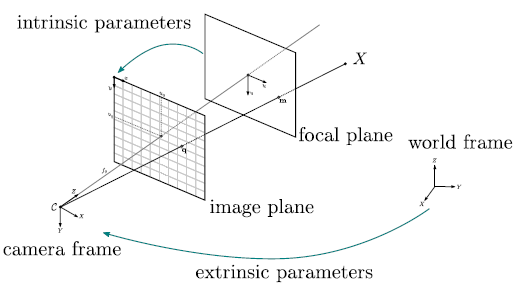
\includegraphics[width=0.7\linewidth]{chapters/camera/image3.png}
\caption{A pinhole-kameramodell.}
\label{fig:pinhole}
\end{figure}
	
	
A kamerához definiálható egy kamera koordináta-rendszer. Ennek a koordináta-rendszernek az origójában van a vetítés középpontja, a z tengelye merőleges a vetítés síkjára. A kép koordináta-rendszer síkbeli koordináta-rendszer, a síkra vetített pontokat értelmezzük ebben. $x$ és $y$ tengelyei a kamera koordináta-rendszer tengelyeivel egyirányúak, és általában $u$ és $v$ betűkkel jelöljük őket, megkülönböztetve őket a kamera koordináta rendszer tengelyeitől. Amennyiben homogén koordinátákkal jellemezzük a tér pontjait, mind a perspektív vetítés, mind a világ koordináta-rendszer és a kamera koordináta-rendszer közötti eltolás, forgatás mátrixszal kifejezhető: 

\begin{align}
\label{eq:cam-trf-basic}
&w \left[ \begin{array}{c} u \\ v \\ 1 \end{array} \right] = \mathbf{A} \; \mathbf{T} \left[ \begin{array}{c} x \\ y \\ z \\ 1 \end{array} \right] \\ \nonumber
&\mathbf{A} = 
\left[ 
\begin{array}{ccc}
f_x & \gamma & u_0 \\
0 & f_y & v_0 \\
0 & 0 & 1
\end{array}
\right] \\ \nonumber
&\mathbf{T} = \left[
\begin{array}{cc}
\mathbf{R} & \mathbf{t}
\end{array}
\right]
\end{align}

Ahol:
\begin{itemize}
\item $u\; v$ a képpont képi koordinátái. $w$ a homogén koordináták miatti komponens
\item $x,\; y,\; z$ a tárgypont koordinátái világ koordináta-rendszerben
\item $\mathbf{A}$ az úgynevezett kameramátrix
\item $f_x, \; f_y$ a kamera fókusztávolsága (ideális esetben egyenlőek, valós alkalmazásokban nem feltétlenül)
\item $\gamma$ egy \textit{skew} nevű torzítási paraméter, ami ideális esetben 0
\item $u_0,\; v_0$ a kamera principális pontjának koordinátái kép koordináta-rendszerben. Ez az a pont, ahol a kamera koordináta rendszer $z$ tengelye döfi a képsíkot
\item $\mathbf{T}$ a világ koordináta-rendszerből kamera koordináta-rendszerbe való transzformáció.
\item $\mathbf{R} \in \mathbb{R}^{3 \times 3}$ forgatási mátrix
\item $\mathbf{t} \in \mathbb{R}^{3 \times 1}$ eltolási vektor
\end{itemize}
 
A kameramátrix paramétereit kamera belső paramétereinek nevezzük. Mivel ezek a kamera rendeltetésszerű használata során nem változnak jelentősen, a kamera szerves részei, egyszeri kalibrálással meghatározhatók. A koordináta-rendszerek közti transzformáció paraméterei a külső paraméterek. Az összes paraméter meghatározható kellően nagy számú pontpár segítségével, ezt kamera-kalibrációnak nevezzük. Pontpárok alatt a világ koordináta-rendszerben ismert pozíciójú pontokat és azok kép koordináta-rendszerben megadott vetületét értjük. A tényleges kalibrációnál általában egy kalibráló objektumról több, különböző nézőpontból készült képet használunk. A kalibráló objektum jellemzően több, egyszerűen, de akár szubpixeles pontossággal detektálható pontból áll, például sakktábla-mintázat sarkai, vagy körökből álló rácsozat pontjainak közepe.

A valóságban a pinhole kameramodell sajnos nem állja meg a helyét, a képet többféle torzítás terheli például abból adódóan, hogy nem vetítést alkalmazunk, hanem lencserendszert, valamint, hogy a detektoron elhelyezkedő pixelek gyártástechnológiája nem tökéletes. Ezeket a paramétereket most nem mutatom be.

Az OpenCV-ben a kamera-kalibráció implementálva van, ami meghatározza mind a belső paramétereket, mind a torzítási paramétereket.

\section{Külső paraméterek meghatározása, PnP probléma}
%TODO módszerek leírása http://iplimage.com/blog/p3p-perspective-point-overview/

	A kamera használata során szükség van a külső paramétereinek ismeretére. Azt a feladatot, amely ismert térbeli helyzetű tárgypontok és a hozzájuk tartozó képi pontok alapján próbálja meghatározni a kamera külső paramétereit PnP, azaz Perspective-n-Point problémának nevezzük. 
	
Ennek egyik verziója a P3P algoritmus \cite{XiaoPnP}, amely csak 4 pontpárból számítja a paramétereket. Három pont kell ahhoz, hogy véges sok megoldást kapjunk (négy ponttal már túlhatározott lenne a feladat). A negyedik pontot az algoritmus arra használja fel, hogy a véges sok megoldás közül kiválassza a helyeset. Ezt úgy teszi meg, hogy a lehetséges négyféle megoldás közül azt választja, amelyikkel a negyedik pontot a képre vetítve a legkisebb hibát kapjuk a megadott képi ponthoz képest. Ezt aztán tetszőleges optimumkereséssel tovább lehet finomítani, pl. Levenberg-Marquardt eljárással. Ezt az eljárást használhatjuk akkor is, ha több, mint négy pont áll rendelkezése.

A PnP probléma megoldása során előfordulhat, hogy hibás pontpárosítások is kerülnek a bemeneti adatok közé. Többek között ennek a kiszűrésére alkalmas a következő szakaszban bemutatott algoritmus.

\section{RANSAC algoritmus}
A RANSAC (Random Sample Consensus) \cite{FischerRANSAC} algoritmus nem kifejezetten képfeldolgozási, hanem általános célú algoritmus, de az általam használt algoritmusok közül többnek részét képezi, ezért indokoltnak tartom bemutatni a működését. A RANSAC módszer annak a problémának egy megközelítése, amikor hibás mérésekkel terhelt adathalmazra próbálunk modellt illeszteni. Itt a modell lehet bármi, ami valamilyen pontossággal illeszkedik az adatokra. Ezt általában 2D ponthalmazra való egyenesillesztéssel szokás szemléltetni. A kiugró mérési hibák miatt jellemzően nem érdemes a legkisebb négyzetek módszerét használni, mert rossz illeszkedést fog mutatni. Ezt szemlélteti a következő ábra.

\begin{figure}[H]
\centering
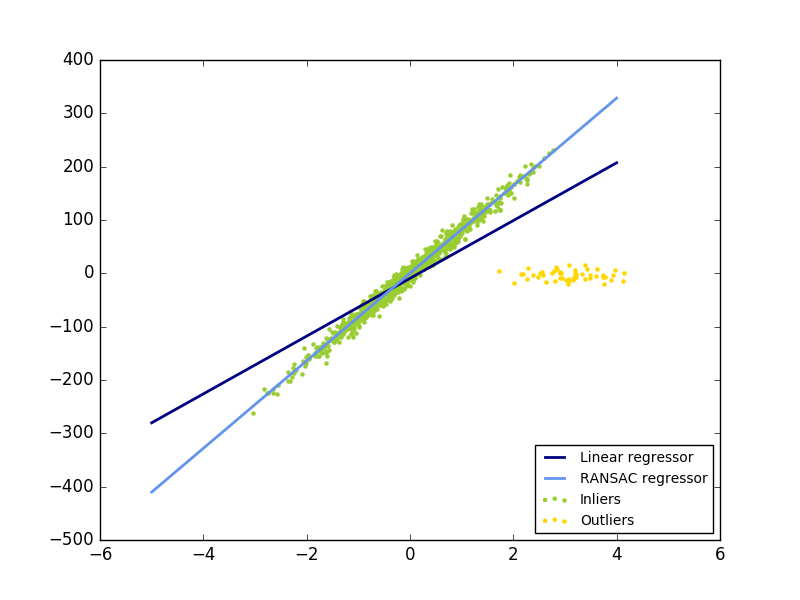
\includegraphics[width=0.7\linewidth]{chapters/camera/ransac.png}
%http://scikit-learn.org/stable/auto_examples/linear_model/plot_ransac.html
\caption{A RANSAC algoritmus és a legkisebb négyzetek módszerének összehasonlítása.}
\label{fig:ransac}
\end{figure}

Az algoritmus leírása során az angol terminológiát használom, a helyes mérési adatot \textit{inlier}-nek nevezem, a mérési hibát pedig \textit{outlier}-nek. 

A RANSAC algoritmus működése a következő:

\vspace{5mm}
\setlength\tabcolsep{0pt}
\noindent \begin{tabularx}{\textwidth}{rlllllllll}
%\noindent \begin{tabularx}{\textwidth}{|l|l|l|l|l|l|l|l|l|l|}
\hline
\multicolumn{10}{c}{\textbf{RANSAC algoritmus}} \\ \hline
1: \hspace{5pt} & \multicolumn{9}{l}{\textbf{eljárás} RANSAC($adatok$, $K$, $e$)} \\
2: \hspace{5pt} & \hspace{20pt} & \multicolumn{8}{l}{\textit{legjobb modell} $\leftarrow$ \textit{null}} \\
3: \hspace{5pt} & \hspace{20pt} & \multicolumn{8}{l}{\textbf{ciklus} $i \leftarrow 1,K$} \\
4: \hspace{5pt} & \hspace{20pt} & \hspace{20pt} & \multicolumn{7}{l}{\textit{vélt inlierek} $\leftarrow N$ darab véletlen adatpont} \\
5: \hspace{5pt} & \hspace{20pt} & \hspace{20pt} & \multicolumn{7}{l}{\textit{vélt modell} $\leftarrow$ \textit{vélt inlierek}-re illesztett modell} \\
6: \hspace{5pt} & \hspace{20pt} & \hspace{20pt} & \multicolumn{7}{l}{\textit{illeszkedők} $\leftarrow$ \textit{vélt modell}-re $e$ hibahatáron belül illeszkedő pontok} \\
7: \hspace{5pt} & \hspace{20pt} & \hspace{20pt} & \multicolumn{7}{l}{\textbf{ha} \textit{illeszkedők} száma $> N$} \\
8: \hspace{5pt} & \hspace{20pt} & \hspace{20pt} & \hspace{20pt} & \multicolumn{6}{l}{\textit{becsült modell} $\leftarrow$ \textit{illeszkedők}-re illesztett új modell} \\
9: \hspace{5pt} & \hspace{20pt} & \hspace{20pt} & \hspace{20pt} & \multicolumn{6}{l}{\textbf{ha} \textit{legjobb modell}-nél jobb \textit{becsült modell}} \\
10: \hspace{5pt} & \hspace{20pt} & \hspace{20pt} & \hspace{20pt} & \hspace{20pt} & \multicolumn{5}{l}{\textit{legjobb modell} $\leftarrow$ \textit{becsült modell}} \\
11: \hspace{5pt} & \hspace{20pt} & \multicolumn{8}{l}{\textbf{visszatérés} \textit{legjobb modell}\textbf{-lel}} \\
\hline
\end{tabularx}
\vspace{5mm}

Az algoritmus robusztussága abban rejlik, hogy ha a 4. sorban a \textit{vélt inlierek} közé nem kerül egyetlen outlier sem, a \textit{vélt modell}-re a legtöbb inlier illeszkedni fog $e$ hibahatáron belül, és a 8. sorban egy nagyon jó illeszkedésű modellt kapunk. Ebben az esetben akár le is lehet állítani az iterálást, és rögtön visszatérni a legjobb modellel.

A RANSAC algoritmus előnye, hogy nagy mennyiségű outlier jelenlétében is képes megtalálni az inlierekre illeszkedő modellt. Létezik olyan verziója is, amellyel 5\% inlier arány mellett is sikeres eredményeket értek el \cite{ransac5}. Hátránya, hogy a véletlenszerű működés miatt nem garantál "optimális" megoldást, és ha meg is találja, a végrehajtási idő véletlenszerűen változhat futásról futásra.
